\chapter{Code Implementation Details}
\section{U-net}
\label{sec:unet}
The section describes the U-Net implementation used in more detail consisting of four classes which are described as follows:
\begin{enumerate}
  \item \textbf{DoubleConv module:} This module consists of two consecutive 3x3 convolutional layers, each followed by batch normalization and a ReLU activation function. This double convolution structure is used to increase the non-linearity of the network but also the receptive field, which allows it to capture more contextual information from the input image.
  \item \textbf{Down module:} This module combines a 2x2 pooling layer with a stride of 2, followed by the DoubleConv module from (1). The max-pooling layer is responsible for reducing the size of the intermediate feature representations and increasing their receptive field.
  \item \textbf{Up module:} This module upsamples the feature representations and concatenates feature maps from the corresponding level in the encoding path. Subsequently, the DoubleConv module from (1) is applied. The upsampling is performed using a transposed convolution where the weights of the convolution kernel are learnable, allowing the network to adapt its upsampling strategy during the training process. Refer to \cite{8618415} for further information on transposed convolution.
  \item \textbf{UNet class:} The primary U-Net model is composed of several layers, which include the DoubleConv module, a set of Down modules from (2) for the encoding path, and a set of Up modules for the decoding path, closing with a final 1x1 convolution layer for mapping the feature maps to the desired number of output classes. \figref{network_architecture} illustrates a detailed representation of the used network architecture.
\end{enumerate}
\figref{uml_unet} provides a more detailed representation of a UML class diagram.
\begin{figure}[H]%[htbp]
  \centering
  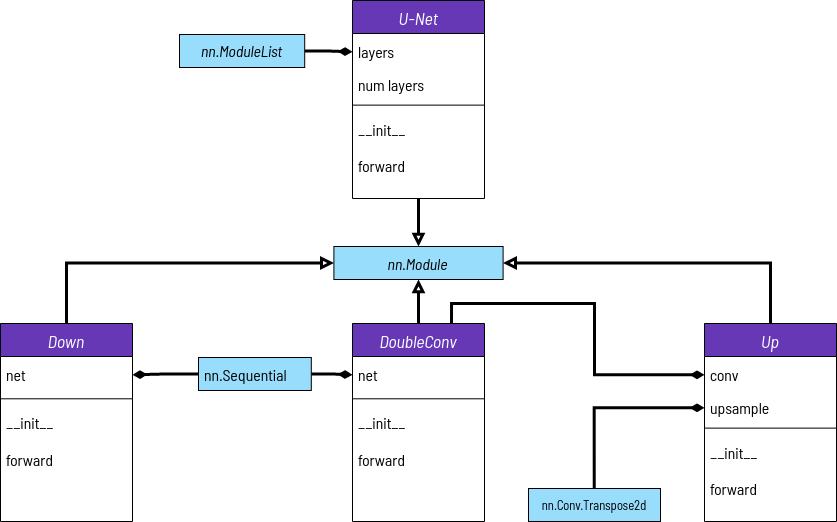
\includegraphics[width=\imgWidthXL]{images/UNET_uml.png}
  \caption[Workstation]{U-Net implementation modeled as a UML diagram. Each class consists of three compartments containing the name, the attributes, and the operations. Solid lines with hollow arrowheads indicate \emph{inheritance}, and a filled diamond shape at the end of the line connecting the \squote{whole} class to the \squote{part} class is called a \emph{composition} \protect\footnotemark.}
  \label{uml_unet}
\end{figure}
\footnotetext{A composition relationship is a strong form of the \squote{whole-part} relationship, where the lifetime of the \squote{part} objects is strictly tied to the lifetime of the \squote{whole} object. In this case, the diamond shape is filled (usually black) and is located at the end of the line connected to the \squote{whole} class. When the \squote{whole} object is destroyed, the \squote{part} objects are also destroyed.}